% CVPR 2023 Paper Template
% based on the CVPR template provided by Ming-Ming Cheng (https://github.com/MCG-NKU/CVPR_Template)
% modified and extended by Stefan Roth (stefan.roth@NOSPAMtu-darmstadt.de)

\documentclass[10pt,twocolumn,letterpaper]{article}

%%%%%%%%% PAPER TYPE  - PLEASE UPDATE FOR FINAL VERSION
% \usepackage[review]{style/cvpr}      % To produce the REVIEW version
% \usepackage{style/cvpr}              % To produce the CAMERA-READY version
\usepackage[pagenumbers]{style/cvpr} % To force page numbers, e.g. for an arXiv version

% Include other packages here, before hyperref.
\usepackage{graphicx}
\usepackage{amsmath}
\usepackage{amssymb}
\usepackage{booktabs}

% If you comment hyperref and then uncomment it, you should delete
% ReviewTempalte.aux before re-running LaTeX.
% (Or just hit 'q' on the first LaTeX run, let it finish, and you
%  should be clear).
\usepackage[pagebackref,breaklinks,colorlinks]{hyperref}


% Support for easy cross-referencing
\usepackage[capitalize]{cleveref}
\crefname{section}{Sec.}{Secs.}
\Crefname{section}{Section}{Sections}
\Crefname{table}{Table}{Tables}
\crefname{table}{Tab.}{Tabs.}


%%%%%%%%% PAPER ID  - PLEASE UPDATE
\def\cvprPaperID{*****} % *** Enter the CVPR Paper ID here
\def\confName{CVPR}
\def\confYear{2023}


\begin{document}

%%%%%%%%% TITLE - PLEASE UPDATE
\title{Handwriting Generation and Animation with Deep Learning}

\author{Anita Dash\\
MA20BTECH11001\\
% For a paper whose authors are all at the same institution,
% omit the following lines up until the closing ``}''.
% Additional authors and addresses can be added with ``\and'',
% just like the second author.
% To save space, use either the email address or home page, not both
\and
Dhruv Srikanth\\
EE20BTECH11014\\
\and
Shambhu Prasad Kavir\\
CS20BTECH11045\\
\and
Taha Adeel Mohammed\\
CS20BTECH11052\\
}

\maketitle

%%%%%%%%% ABSTRACT
\begin{abstract}
   Handwriting style transfer for personalized text generation is a fascinating and evolving field that sits at the intersection of computer vision and natural language processing. It has several applications in various domains, ranging from enhancing digital communication and marketing to improving accessibility and education.

   In this project, we aim to create a system that takes a written text prompt and a sample of the handwriting to mimic as the input, and generates realistic animated handwritten text that closely resembles the provided style while maintaining readability and coherence.
\end{abstract}

\section{Introduction}
\label{sec:introduction}
% intro, motivation
Handwriting is a deeply personal and authentic form of expression. It holds a unique place in human communication and self-expression. In this regard, Handwriting Style Transfer can come in handy. A model that generates handwritten text in a particular style can be helpful in the following fields:-
\begin{itemize}
    \item In education, personalized handwritten materials can improve student engagement and retention, offering educators a powerful tool to make learning more effective and enjoyable.
    \item Handwriting style transfer can improve accessibility for individuals with motor disabilities, allowing them to convey their thoughts and emotions through personalized handwriting styles, promoting inclusivity in communication.
    \item Handwritten image generation can also provide additional data to train more accurate general handwriting recognition models 
    \item It can help in the field of forensic analysis such as forgery detection, document authentication etc.
    \item Businesses can leverage personalized handwriting in marketing materials, enhancing customer engagement, and creating memorable brand experiences.
\end{itemize}

% the model
% base model
\section{Problem Statement}
\label{sec: PS}
Implement a deep learning model that can take a text prompt and a sample image of a person's handwriting style as input, and generate the image of the text prompt, in the specified handwriting style as the output. We want the model to accurately mimic the unique characteristics, nuances, and idiosyncrasies of the provided handwriting style while maintaining the readability and coherence of the generated text. We could consider further diversification - calculating the temporal sequence of brush strokes: if our generation model is successful, we could try to calculate the pen trajectory, i.e. the successive coordinate points for every time step of the brush stroke, to be extracted. This trajectory can then be used to animate the brush stroke in real-time, creating a realistic animated handwritten text.  


\section{Literature Review}
\label{sec: Lit Rev}
There has been a lot of research in the field of handwriting generation and handwriting trajectory recovery. In this section, we discuss the various models and approaches that have been proposed in the literature to solve these problems. We then aim to combine these state-of-the-art techniques to create a model that can generate realistic animated handwritten text in a particular style.

\subsection{Decoupled Style Descriptors} 
\label{subsec: Brush Paper}
 Capturing a space of handwriting stroke styles poses the challenge of representing both the style of each character and the overall style of the human writer.
This paper~\cite{BRUSH-paper} introduces an approach to online handwriting stroke representation via the Decoupled Style Descriptor (DSD) Model. 

As handwriting strokes can be modeled as  a sequence of points over time, supervised deep learning methods to handwriting representation can use recurrent neural networks (RNN).

In this approach, there are three variations represented within an RNN model: the variation in writer style, the variation in character style, and the variation in writer-character style. Given a database of timestamped sequences of handwriting strokes with character labels, this model learns a representation that encodes three critical factors:- writer-independent character descriptors, writer-dependent character string style descriptors and writer-dependent global style descriptors.

We have as input $x = (p_1, p_2, ... p_N)$ which represents the stroke sequence and $s = (c_1, c_2, ..., c_M)$ represents the character sequence. An unsupervised learning technique is used to train a segmentation network $k_{\theta}(x,s)$ to map regions in $x$ to characters.
 We wish to predict $x'$ comprised of $p'_t$.  Further, Mixed Density Networks are used to provide variation in the output while generating the writing.

For the given $x, s$ and a target string $c_t$ a parameterized encoder function $f^{enc}_{\theta}$ is trained to learn writer-dependent character-dependent latent vectors $w_{c_t}$. Simultaneously, a parameterized decoder function $f^{dec}_{\theta}$ is trained to predict the next point $p'_t$ given all the past points $p'_{1:t-1}$. Both the encoder and decoder functions used here are RNNs. To this method, so as to factor in character-independent writer style, we add another layer of abstraction, and introduce a parameterized encoder function $g_{\theta}$. 
% \begin{itemize}
%   \item When two stroke sequences $x_1$ and $x_2$ are written by the same writer, consistency in their writing style is represented by a character-independent writer-independent later vector $w$
%   \item When two character sequences $s_1$ and $s_2$ are written by the different writer, consistency in their writing style is represented by a character-dependent writer-independent latent matrix $C$, which is estimated using a parameterized encoder function $g_{\theta}$, also an RNN. 
%   \item $C_{c_t}$ instantiates a writer's style to draw a character via $w_{c_t}$, such that $C_{c_t}$ and $w$ are latent factors.
% \end{itemize} 

Given a target character $c_t$, we use encoder $g_{\theta}$ to generate a $C$ matrix. We then multiply $C_{c_t}$ by a desired writer style $w$ to generate $w_{c_t}$. Finally, we use a trained decoder $f^{dec}_{\theta}$ to create a new point $p'_t$ given previous points $p'_{1:t-1}$.
\begin{equation*}
  p'_t = f^{dec}_{\theta}(p'_{1:t-1}|w_{c_t}), \text{where } w_{c_t} = C_{c_t}w
\end{equation*}
In a qualitative user study, it was observed that the drawing samples generated by this model were preferred over few of the state of the art techniques. Further the model was also successful in interpolating samples at different levels, recovering representations for new characters and achieved high-writer identification accuracy. Despite that, the model occasionally failed in producing legible letters or in connecting cursive letters. One of the causes for this issue being the underlying inconsistencies in human writing, which was only partially addressed in this model. Additionally, the process of collecting high-quality data using digital pens in a crowdsourced environment, involving careful data cleaning, persists to be another challenge. 


\subsection{GANwriting}
\label{subsec: GANWriting}
Generative Adversarial Networks (GANs) have been succesfully used for generating illusory plausible images in various fields. GANs consist of two neural networks, a generator, and a discriminator, which are trained simultaneously through a competitive process in which both improve iteratively. 

In the paper~\cite{GAN-1}, the authors use a conditional non-recurrent generative adversial (cGAN), to produce realistic handwritten word images. In order to produce these diverse stylized words, the textual content along with the specific wrting style, defined by a latent set of calligraphic attributes, are separately conditioned on the generative model. To train the model and achieve the desired results, the authors used the following three novel techniques:
\begin{itemize}
    \item Three complementary learning objectives, namely adversial loss, style classification loss, and reconstruction loss, are used to train the model. State-of-the-art discriminator, classifier, and word recognizer networks are used to train the model.
    \item Character-based content conditioning is done, allowing to generate any word, without being restricted to a specific vocabulary.
    \item Few-shot calligraphic style conditioning is done to avoide the mode collapse problem.
\end{itemize}


However this model is limited to singular words. In the paper~\cite{GAN-2}, they expand on these ideas to allow variable length  textual input, allowing it to generates entire lines of offline handwriting.

\subsection{Handwriting Transformers}
\label{subsec: HWT}
Earlier Handwriting generative methods process style and features separately. It doesn't encode style content entanglement at a character level. In this paper ~\cite{HWT}. the authors propose a transformer-based styled handwritten text image generation approach, HWT, that strives to learn both style-content entanglement as well as global (such as ink width, slant) and local (such as character style, ligatures) writing style patterns. The overall architecture has four components: 
\begin{itemize}
  \item Conditional Generator : Synthesize handwritten text.
  \item Discriminator: Ensures realistic generation of handwriting styles. It is designed to be convolutional in nature
  \item Recognizer: Aids in textual content preservation. It is inspired by CRNN
  \item Style Classifier: Ensures satisfactory transfer of calligraphic styles.
\end{itemize}

In the paper, the focus of the design is in the generator model. To imitate a handwriting style as realistically as possible, This model is designed to learn style content entanglement as well as local and global style patterns.  It is a transformer-based generative network for unconstrained styled handwritten text image generation.  It has two main components an encoder network and a decoder network.  Both the encoder and decoder networks constitute a hybrid design based on convolution and multi-head self-attention networks.

HWT generates realistic styled handwritten text images and significantly outperforms other state-of-the-art models through extensive qualitative, quantitative and human based evaluations. The model also generalizes well to the challenging scenarios where both words and writing style are unseen during training, generating realistic styled handwritten text images 

\subsection{Dynamically configurable CRNN (Recognizer)}
\label{subsec: CRNN}

The DC-CRNN (Dynamically Configurable Convolutional Recurrent Neural Network) \cite{crnn} is one of the best performing handwriting recognition models out now. The CRNN has been used as a recognizer in other models as well. Recognition is a vital prerequisite to generation so we can learn how to better generate handwritten text from better recognition models.

The CRNN structure counters the most significant challenge with handwriting analysis which is variable-length sequences. A CNN module is used to extract spatial features while the label, text data corresponding to the image, is treated as a character sequence fed to the RNN. With this setup, the model is able to accurately learn correlation between different characters while considering the global effect of the handwriting style via its CNN module. The optimization problem is framed differently using SSA and LAHC to have a more generalized solution that considers more of the data than exploit it using swarm optimization given the complexity of the latent space. Though the algorithm itself requires more investigation to understand its specific value, the result is shown to significantly improve when LAHC (Late Acceptance Hill Climbing) is used - comparing current solution with that from multiple steps ago to ensure stability.

Other models are limited by the sequence and this architecture appears to solve that long-standing issue. We want to explore possible integration of these techniques in generation models for improved performance.

\subsection{Handwriting Trajectory Recovery}
\label{subsec: img2stroke}
Temporal information is unavailable when it comes to offline text. An image scanner or a video camera is not capable of extracting information like velocity, pressure, inclination etc. If one is able to recover the stroke trajectory from the static 2D image, then offline text can be viewed as an online text. This paper \cite{image2stroke-1Char} proposes a technique that can predict the probable trajectory of an offline character level image.

The model is inspired from the sequence to sequence model based on encoder-decoder architecture. The model sequentially predicts the data coordinate points of the pen trajectory from the offline character images.The framework of this model consists of mainly two steps.
\begin{itemize}
    \item Extract a sequence feature vector from the offline images using CNN.
    \item  An encoder-decoder LSTM network takes the sequence feature as the input and outputs the required coordinate points.
\end{itemize}

The model is able to find out the correct starting point and extract the correct incoming and outgoing paths from junction points effectively. 


\subsection{Domain-Adversarial Neural Network}
\label{subsec: DANN}

DANN (Domain-Adversarial Neural Network) \cite{DANN} is an interesting architecture that we believe, could be utilized in the problem of specific-style handwriting generation. DANN is an improvement to any regular network structure due to its parallel branch.

Given a Neural Network performing a downstream task on a given dataset, the output of the penultimate layer is considered the final representation of the input data. On this representation, we apply our last layer which is the downstream task itself but the more interesting part is the learnt representation. We claim that with enough training, this penultimate layer output is the best possible latent space representation of the data distribution possessing the information required to perform a downstream task. The nature of Deep Learning makes it so that we can never truly know the kind of correlations the model has learnt from the input data and how the information is being represented but we know that the information required for the downstream task is somehow contained in the representation. If the existence of a downstream task and its loss function controls the information present in the representation, then if we want to include or exclude further information from the representation, all we need to do is have a parallel branch of the neural network performing that downstream task on the representation. When we consider the loss of this new branch downstream task while updating our representation-learning, the learnt representation now possesses or is independent of information regarding this task.

For example, if we had images of X-Rays of a human body part and we had to determine if the subject is fractured or not, our primary downstream task would be to classify the image as fractured or not. But if we have labels as to what part of the human body is present in the image, then we can ensure that our representation learns features of the image that are independent of whether the subject is a hand or a leg. This can be implemented by having a parallel downstream task on the representation that classifies the image as being an X-Ray of a hand or an X-Ray of a leg. Next, we subtract the loss of this classifier for the representation-learning layers. Thus, the model is forced to get worse at identifying whether the subject in the image is a hand or a leg making its learnt representation independent (but aware) of this information and only focussed on whether the subject is fractured or not.

Thus, this architecture allows us to hand-pick the kind of information we want to be depicted in the model's latent space representation of the data by making the model either improve or become worse at a parallel task involving correlated information. This architecture was originally proposed for use in the biomedical space but we believe that style transfer problems too could benefit from such an architecture due to the requirement of considering handwriting style information and character information distinctly. If we are able to isolate the style information from the character information completely giving the model a better empirical understanding of the handwriting style itself, this may improve our ability to generate better handwriting samples.

\subsection{Writing Order Recovery}
Writing order recovery is a complex problem that relates to the intrinsic properties of human handwriting. However, integrating its solution with an observed handwritten text could tell us more about a subject's characteristic handwriting than ever before. This paper \cite{WOR} proposes an innovative deterministic algorithm to recover the writing order of any thinned long static handwritten signature. Signatures have been chosen out of the belief that they are the most complex version of this problem.

The proposed method is completely intuitive and draws from the good continuity criteria of handwriting. The process of recovery has been split into 3 subprocesses - point classification, local examination, and global reconstruction.
Strokes are believed to be entirely continuous so the authors have observed the 8-connected pixels, adjacent pixels surrounding a target pixel, to observe the target pixel's position within a stroke. A pixel with 2 connected pixels is believed to be a trace-point, one of the points along the trajectory of a stroke. A point with only 1 connected pixel is believed to be an end-point of a stroke. Any point with more than 2 connected pixels is believed to be a cluster point, a point found in the region of overlap between 2 distinct strokes/components.
After this classification, the next step is described as local examination. Adjacent trace points are considered to be part of one stroke and hence form large groups reconstructing the strokes from an end-point, through trace-points, to another end-point. The only complexity remaining at this stage is that of overlapping strokes forming clusters. Branches exiting clusters are marked with anchor points and their exit angles are measured and characterized. The authors define a few commonly occurring cluster scenarios and match the present observed cluster to the predefined scenarios.
In the global reconstruction stage, clusters are resolved by modelling the rapid change in direction (from branch angle and position) as energy alongside assigning priority to each branch and each scenario to perform energy minimization. After the internal cluster paths are separated, the authors use a Gaussian spread formulation to choose the leftmost starting point of a stroke and use a proximity criterion to connect a pen-up point to the next pen-down point thus deriving the order of strokes/components.

The main complexity of such a problem has been described as the interpolation of pen-up and pen-down amidst strokes causing distinct strokes and consequently their overlap. The solution proposed to this problem is intuitive and replicative of a human thought process which is why it captured our attention. Obtaining the temporal properties has been left as a future problem that could, in their opinion, aid more significantly in the field of handwriting recognition, analysis, and generation.

\section{Replicated Results}

GANwriting \cite{GAN-1} is limited to generating singular words, and as a result we cannot have outputs of variable length. This is a major drawback as we want to generate entire lines of text. It doesn't encode style content entanglement at a character level and hence struggles to mimic character specific styles.\\

\begin{figure}[h]
  \centering
  \begin{subfigure}[b]{0.45\textwidth}
    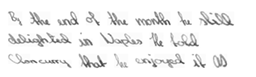
\includegraphics[width=\textwidth]{../latex-src/Images/Gan-Input1.png}
    \caption{\textbf{Desired Handwriting}}
    \label{fig:GAN-input}
  \end{subfigure}
  \hfill
  \begin{subfigure}[b]{0.45\textwidth}
    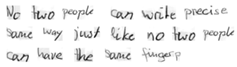
\includegraphics[width=\textwidth]{../latex-src/Images/Gan-Output1.png}
    \caption{\textbf{GANwriting}}
    \label{fig:GAN-output}
  \end{subfigure}
  \caption{{Since GANwriting is limited to generating fixed number of words, it fails to generate the entire line of text. It also fails to capture the style of the text.}}
  \label{fig:GAN}
\end{figure}

While Decoupled Style Descriptors \cite{BRUSH-paper} is able to capture local and global style patterns, it fails to generate legible letters or connect cursive letters. This is because of the underlying inconsistencies in human writing, which is only partially addressed in this model. Additionally, the model works with online handwriting data and we want to capture the styles of offline handwriting.

Handwriting Transformers \cite{HWT} is able to generate realistic styled handwritten text images and significantly outperforms other state-of-the-art models. It handles variable length input and captures local and global style patterns. It is also compatible with offline handwriting data. Hence we have decided to use this model as our base model.\\

\begin{figure}[h]
  \centering
  \begin{subfigure}[b]{0.45\textwidth}
    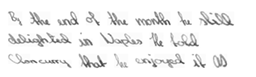
\includegraphics[width=\textwidth]{../latex-src/Images/Gan-Input1.png}
    \caption{\textbf{Desired Handwriting}}
    \label{fig:HWT-input}
  \end{subfigure}
  \hfill
  \begin{subfigure}[b]{0.45\textwidth}
    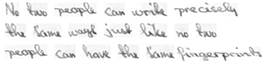
\includegraphics[width=\textwidth]{../latex-src/Images/HWT-Output1.png}
    \caption{\textbf{HWT}}
    \label{fig:HWT-output}
  \end{subfigure}
  \caption{{HWT is able to generate the entire line of text. It also captures the local and global style of the text.}}
  \label{fig:HWT}
\end{figure}
\subsection{FID Scores}
The Fréchet Inception Distance (FID) is a metric used to evaluate the quality of generated images. It is based on the Inception Score (IS) and the Frechet Distance (FD).It is a metric that measures the similarity between two distributions. The FID score is the Frechet Distance between the distribution of the real images and the distribution of the generated images. The lower the FID score, the better the quality of the generated images. A score close to zero implies that the two groups of images are nearly identical. \newline
\newline
\textbf{Table 1: Comparison of HWT with GANwriting model} with respect to their FID scores computed between the generated text images and the real text images from the IAM dataset. We generate datasets of 6 images each for both the models. The FID score for the HWT model is lower than that of the GANwriting model implying that the former generates better quality images than the latter.
\begin{table}[h]
  \begin{center}
    \begin{tabular}{|c|c|}
      \hline
      \textbf{Model} & \textbf{FID Score} \\
      \hline
      HWT & 70.67 \\
      \hline
      GANwriting & 94.77 \\
      \hline
    \end{tabular}
  \end{center}
% \caption{FID scores for HWT and GANwriting models}
\end{table}\\
While the size of the datasets used here was rather small, we can still observe that the HWT model generates better quality images than the GANwriting model. This is because the HWT model is able to capture the local and global style patterns of the text, while the GANwriting model is not. The purpose of this test was only to attest what was already proven in the papers. 
\newline
\textbf{Table 2: Comparison of HWT model with ScrabbleGAN and Davis et al} with respect to their FID scores. We generate a dataset of 95 images for the HWT model and then compute its FID score. For the other models, we take the FID scores as mentioned in the paper. Once again, we observe that the HWT model has a lower FID score than the other models. 
\begin{table}[h]
  \begin{center}
    \begin{tabular}{|c|c|}
      \hline
      \textbf{Model} & \textbf{FID Score} \\
      \hline
      HWT & 16.71 \\
      \hline
      ScrabbleGAN & 20.72 \\
      \hline
      Davis et al & 20.65 \\
      \hline
    \end{tabular}
  \end{center}
\end{table} \\
Since we have used a significantly smaller dataset for computing the FID score for the HWT model, the results may not be entirely accurate. However, we can still observe that the HWT model has a lower FID score than the other models.
\subsection{Testing}
Add results
\section{Preliminary Results}
Testing with our own handwriting \\
Add changes made to make testing more accessibile 
%%%%%%%%% REFERENCES
{\small
\bibliographystyle{style/ieee_fullname}
\bibliography{references/ppr-references}
}

\end{document}
